Một trường hợp đặc biệt giúp minh họa rõ ý nghĩa của ba khái niệm xấp xỉ là khi
\[
F=\iota_C,
\]
trong đó $\iota_C$ là hàm chỉ báo của một tập lồi đóng
$C\subset\Hil$, tức
\[
\iota_C(x)=
\begin{cases}
0, & x\in C,\\
+\infty, & x\notin C.
\end{cases}
\]
Khi đó bài toán điểm gần kề trở thành bài toán chiếu trực giao lên $C$, vì
\[
\prox_{\lambda F}=P_C,
\]
không phụ thuộc vào tham số $\lambda$.
\begin{essayonly}
Do đó, ba khái niệm xấp xỉ của điểm gần kề có thể được diễn giải hoàn toàn bằng hình học, giúp thấy rõ sự khác biệt giữa chúng.
\end{essayonly}

\paragraph{Xấp xỉ loại 1.}
Từ định nghĩa của xấp xỉ loại~1 và tính chất của phép chiếu trực giao, ta suy ra
\begin{equation}
  z\approx_1 P_C(y)\quad\text{với $\eps$-chính xác}
  \iff
  z\in C
  \text{ và }
  \norm{z-y}^2
  \le
  d(y,C)^2+\eps^2.
  \label{eq:proj-type1}
\end{equation}

\begin{figure}[H]
    \centering
    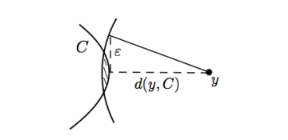
\includegraphics[width=0.5\linewidth]{figures/proj-type1.png}
    \caption{Minh họa xấp xỉ loại~1. Điểm $z$ chỉ cần nằm trong phần tô đậm, tức giao của tập $C$ với hình cầu tâm $y$ có bán kính $\sqrt{d(y,C)^2+\eps^2}$. Vì vậy, $z$ không nhất thiết phải nằm gần điểm chiếu $P_C(y)$.}
    \label{fig:loai_1}
\end{figure}

\begin{essayonly}
Nói cách khác, thay vì yêu cầu $z$ phải là hình chiếu chính xác của $y$ lên $C$, ta chỉ đòi hỏi khoảng cách từ $y$ đến $z$ không vượt quá khoảng cách tối ưu $d(y,C)$ quá một lượng $\eps$. Vì vậy, tập các điểm xấp xỉ loại~1 chính là giao của tập $C$ với hình cầu tâm $y$ có bán kính $\sqrt{d(y,C)^2+\eps^2}$.
\end{essayonly}

\paragraph{Xấp xỉ loại 2.}

Trong trường hợp $F=\iota_C$, điều kiện \eqref{eq:AT2} tương đương với
\begin{equation}
  z\approx_2 P_C(y)\quad\text{với $\eps$-chính xác}
  \iff
  z\in C
  \text{ và }
  \iprod{x-z}{y-z}
  \le
  \frac{\eps^2}{2},
  \quad \forall x\in C.
  \label{eq:proj-type2}
\end{equation}

\begin{essayonly}
Điều kiện trên có thể được hiểu như một sự nới lỏng của đặc trưng hình học đối với phép chiếu trực giao. Điểm chiếu chính xác
$P_C(y)$ được đặc trưng bởi
\[
\iprod{x-P_C(y)}{y-P_C(y)}\le0,
\qquad \forall x\in C,
\]
nghĩa là toàn bộ tập lồi $C$ nằm trong một nửa không gian được xác định bởi siêu phẳng tiếp xúc với $C$ tại $P_C(y)$.

Đối với xấp xỉ loại~2, bất đẳng thức trên được thay bằng
\[
\iprod{x-z}{y-z}\le\frac{\eps^2}{2},
\]
cho phép toàn bộ tập $C$ vượt qua siêu phẳng tiếp xúc một lượng hữu hạn phụ thuộc vào $\eps$. Cụ thể, $C$ chỉ cần nằm trong nửa không gian giới hạn bởi siêu phẳng affine
\[
h_\eps:
\Big\langle
x-z,\,
\frac{y-z}{\norm{y-z}}
\Big\rangle
=
\frac{\eps^2}{2\norm{y-z}},
\]
là siêu phẳng vuông góc với vectơ $y-z$ và song song với siêu phẳng tiếp xúc chính xác. So với trường hợp $\eps=0$, siêu phẳng này được tịnh tiến theo hướng từ $z$ tới $y$ một khoảng
\[
\frac{\eps^2}{2\norm{y-z}}.
\]
\end{essayonly}
\begin{figure}[H]
    \centering
    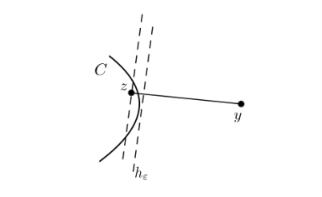
\includegraphics[width=0.5\linewidth]{figures/proj-type2.png}
    \caption{Minh họa xấp xỉ loại 2. Siêu phẳng $h_0$ là siêu phẳng đỡ chính xác tại $z$, còn $h_\varepsilon$ là siêu phẳng song song thu được bằng cách tịnh tiến $h_0$ về phía $y$ một khoảng $\varepsilon^2/(2\|y-z\|)$. Điều kiện \eqref{eq:proj-type2} yêu cầu toàn bộ tập lồi $C$ vẫn nằm trong nửa không gian giới hạn bởi $h_\varepsilon$.}
\label{fig:type2}
\end{figure}

\paragraph{Xấp xỉ loại 3.}
Theo đặc trưng \eqref{eq:AT3-equiv}, xấp xỉ loại~3 của phép chiếu được mô tả bởi
\begin{equation}
  z\approx_3 P_C(y)\quad\text{với $\eps$-chính xác}
  \iff
  z=P_C(y+e),\qquad \norm{e}\le\eps.
  \label{eq:proj-type3}
\end{equation}

\begin{essayonly}
Nói cách khác, thay vì làm tròn trực tiếp điểm chiếu, ta cho phép điểm đầu vào $y$ chịu một nhiễu có chuẩn không vượt quá $\eps$, rồi thực hiện phép chiếu chính xác. Vì vậy, mọi xấp xỉ loại~3 đều là ảnh chiếu của một điểm nằm trong hình cầu tâm $y$, bán kính $\eps$.
\end{essayonly}

\begin{figure}[H]
    \centering
    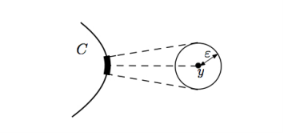
\includegraphics[width=0.5\linewidth]{figures/proj-type3.png}
    \caption{Xấp xỉ loại~3: các điểm xấp xỉ là ảnh chiếu của các điểm trong hình cầu $B(y,\eps)$, do đó luôn nằm trên biên của $C$.}
    \label{fig:type_3}
\end{figure}

\begin{remark}
Một điểm đáng chú ý là, đối với các tập lồi bị chặn, xấp xỉ loại~3 luôn kéo theo xấp xỉ loại~2. Nói cách khác, nếu một điểm là hình chiếu chính xác của một điểm bị nhiễu không quá $\eps$, thì nó đồng thời cũng thỏa điều kiện siêu phẳng của xấp xỉ loại~2 với một sai số lớn hơn nhưng vẫn được kiểm soát tường minh.

\begin{essayonly}
Cụ thể, nếu
\[
z\approx_3P_C(y)
\quad\text{với độ chính xác }\eps,
\]
thì
\[
z\approx_2P_C(y)
\quad\text{với độ chính xác }
\sqrt{2\,\diam(C)\,\eps}.
\]

Thật vậy, theo đặc trưng của xấp xỉ loại~3 trong
\eqref{eq:proj-type3}, tồn tại một vectơ nhiễu
$e\in\Hil$ sao cho
\[
z=P_C(y+e),\qquad \|e\|\le\eps.
\]
Vì $z$ là hình chiếu của $y+e$ lên $C$, nên từ đặc trưng biến phân của phép chiếu suy ra
\[
\langle x-z,\,(y+e)-z\rangle\le0,
\qquad \forall x\in C.
\]
Do đó,
\[
\begin{aligned}
\langle x-z,\;y-z\rangle
&=\langle x-z,\,(y+e)-z\rangle-\langle x-z,e\rangle\\
&\le -\langle x-z,e\rangle\\
&\le \|x-z\|\,\|e\|,
\end{aligned}
\]

Mặt khác, vì cả $x$ và $z$ đều thuộc $C$ nên
$
\|x-z\|\le\diam(C).
$
Kết hợp với $\|e\|\le\eps$ thu được
\[
\langle x-z,\;y-z\rangle
\le
\diam(C)\,\eps,
\qquad \forall x\in C.
\]
So sánh với điều kiện đặc trưng của xấp xỉ loại~2 trong
\eqref{eq:proj-type2},
\[
\langle x-z,\;y-z\rangle
\le
\frac{\eps'^2}{2},
\]
chỉ cần chọn
$
\eps'
=
\sqrt{2\,\diam(C)\,\eps}.
$
\end{essayonly}
\end{remark}
